\documentclass[a4paper,titlepage,11pt]{ltjsarticle}
\usepackage[dvipdfmx]{graphicx}
\usepackage{color}
\usepackage{amssymb}
\usepackage{here}
\usepackage{subcaption}
\usepackage{amsmath}
\usepackage{listings}
\lstset{
	%プログラム言語(複数の言語に対応,C,C++も可)
	language = C,
	%背景色と透過度
	backgroundcolor={\color[gray]{.90}},
	%枠外に行った時の自動改行
	breaklines = true,
	%自動改行後のインデント量(デフォルトでは20[pt])	
	breakindent = 10pt,
	%標準の書体
	basicstyle = \ttfamily\scriptsize,
	%コメントの書体
	commentstyle = {\itshape \color[cmyk]{1,0.4,1,0}},
	%関数名等の色の設定
	classoffset = 0,
	%キーワード(int, ifなど)の書体
	keywordstyle = {\bfseries \color[cmyk]{0,1,0,0}},
	%表示する文字の書体
	stringstyle = {\ttfamily \color[rgb]{0,0,1}},
	%枠 "t"は上に線を記載, "T"は上に二重線を記載
 %他オプション:leftline,topline,bottomline,lines,single,shadowbox
	frame = TBrl,
	%frameまでの間隔(行番号とプログラムの間)
	framesep = 5pt,
	%行番号の位置
	numbers = left,
 %行番号の間隔
	stepnumber = 1,
 %行番号の書体
	numberstyle = \tiny,
 %タブの大きさ
	tabsize = 4,
	%キャプションの場所("tb"ならば上下両方に記載)
	captionpos = t
}

\title{情報システム工学実験Ⅱ\\フルレポート\\画像処理(松岡担当)}
\author{氏名:関川 謙人\\学籍番号:2022531033}
\date{提出日:\today}

\begin{document}
\section{目的}
この講義は授業当日の課題に取り組んで簡単な画像処理を実装することで、日常で使われる画像処理の仕組みやアルゴリズムについて理解することを目的とする。
\section{演習概要}
今回取り組んだ課題は、以下のとおりである。
\begin{table}[h]
	\caption{課題演習}
	\label{table:ex}
	\centering
	\begin{tabular}{|c|c|c|}
		\hline
		課題番号               & 画像処理技術 & 処理
		\\\hline\hline
		\begin{tabular}{l}
			1
			\\\hline
			2
			\\\hline
			3-1
			\\
			\\\hline
			3-2
			\\
			\\\hline
			4
			\\
			\\
			\hline
			5
			\\
			\\
			\\
		\end{tabular} &
		\begin{tabular}{l}
			線形量子化     \\
			\hline
			二値化処理     \\
			\hline
			平均値を用いた縮小 \\
			\\
			\hline
			線形補完法     \\
			\\\hline
			ガウシアンフィルタ
			\\
			\\\hline
			ラプラシアンフィルタ
			\\\hline
			鮮鋭化
			\\
			\\
		\end{tabular} &
		\begin{tabular}{l}
			画素値の階調の数を減らし、データ量を減らす。
			\\\hline
			閾値を基準に、入力画素の値を0か255に置き換える。
			\\\hline
			縮小倍率$\times$縮小倍率の範囲毎に平均値を求め、\\それを出力画素値として出力する。
			\\\hline
			拡大の際に生じる欠損画素を、画素間の画素値が線形に\\変化していると仮定して補う。
			\\\hline
			周辺画素$\times\exp(-2\frac{k^{2}+l^{2}}{2\omega^{2}})$との平均を求め,画像を平滑化する。 \\
			$\omega$は画素値の標準偏差。
			\\\hline
			エッジの抽出。
			\\\hline
			入力画素にラプラシアンフィルタで抽出したエッジを足し込み、                                        \\
			エッジがはっきりとした画像を作る。
		\end{tabular}
		\\\hline
	\end{tabular}
\end{table}
\section{演習課題}
\subsection*{課題1:画像の量子化}
講義で配布した画像ファイル”lena256.ppm”を用いて,線形量子化処理を実行
し,その結果をレポートに貼りつけよ.ただし,任意の N-bit に量子化できるようにプロ
グラムを作成すること.N=2,4,7 のときの量子化結果を比較し考察せよ.

プログラム:
\begin{lstlisting}
	void quantize(ColorImage *outimage, const ColorImage *inimage)
{
 	int <variable>i,j,k;
	int bit_shift;
	printf("何ビットに量子化しますか?\n>>>");
	scanf("%d",&bit_shift); // 量子化ビット
	for(i = 0;i < inimage -> height; i++){
		for(j = 0; j < inimage -> width; j++){
			//量子化処理
			outimage -> r[i][j] = (255/(pow(2,bit_shift)-1))*round(inimage -> r[i][j] /(255/(pow(2,bit_shift)-1)));
			outimage -> g[i][j] = (255/(pow(2,bit_shift)-1))*round(inimage -> g[i][j] /(255/(pow(2,bit_shift)-1)));
			outimage -> b[i][j] = (255/(pow(2,bit_shift)-1))*round(inimage -> b[i][j] /(255/(pow(2,bit_shift)-1)));
		}
	}
}
\end{lstlisting}

実行結果:\\
N=7,N=4,N=2といった風に量子化ビット数が下がっていくにつれて、
画像が粗くなっているのが確認できる。
%画像並べ
%横に4枚の画像(jpg/png)表示
\begin{figure}[H]
\begin{center}
\begin{tabular}{c}
\begin{minipage}{0.25\hsize}
\begin{center}
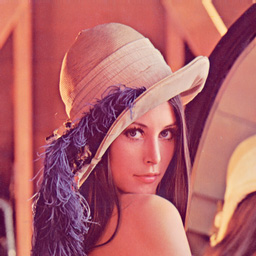
\includegraphics[width=4cm]{lena256.jpg}
\end{center}
\caption*{元画像}
\end{minipage}
\begin{minipage}{0.25\hsize}
\begin{center}
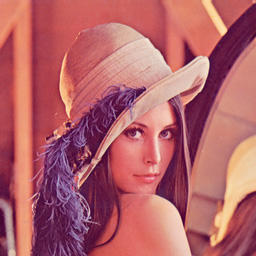
\includegraphics[width=4cm]{quantize_7bit.jpg}
\end{center}
\caption*{N=7}
\end{minipage}
\begin{minipage}{0.25\hsize}
\begin{center}
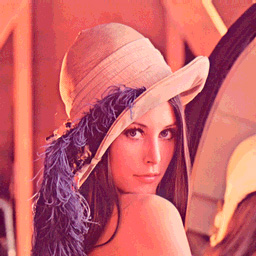
\includegraphics[width=4cm]{quantize_4bit.jpg}
\end{center}
\caption*{N=4}
\end{minipage}
\begin{minipage}{0.25\hsize}
\begin{center}
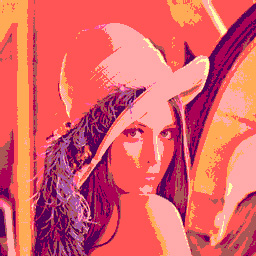
\includegraphics[width=4cm]{quantize_2bit.jpg}
\end{center}
\caption*{N=2}
\end{minipage}
\end{tabular}
\end{center}
\end{figure}

%ここまで画像
考察:\\
入力画像を$f(i,j)$、出力画像を$g(i,j)$とすると、この処理は、
\begin{equation}
	g(i,j)=\frac{255}{2^{N}-1}\times round\Big(\frac{2^{N}-1}{255}f(i,j)\Big)
\end{equation}
となる。

この時$\frac{255}{2^{N}-1}$で基準となる値を決めている。例えばN=2であるとき、
基準値は85である。また、$round(\frac{2^{N}-1}{255}f(i,j))$
の計算式でその画素をどの値とみなすかを決定している。

画素値は基準値の整数倍となりN=2の場合、
(0,85,170,255)のいずれかの値になる。

このときビット数が低くなるにつれて、画素値の種類が少なくなるので画像は粗くなる。

\subsection*{課題2:画像の二値化}
講義で配布した画像ファイル”peppers.ppm”を用いて,以下の処理を実行し,そ
の結果をレポートに貼りつけよ.ただし,2値化の結果が最も良くなる閾値を探し,その
結果を閾値の値とともに報告すること.また,2値化の精度を向上するための方法を考察
せよ.
\\・画像中の緑色のピーマンの領域を2値化で抽出せよ.
\\・画像中の赤色のピーマンの領域を2値化で抽出せよ.
\\

プログラム:
\begin{lstlisting}
	/*2値化*/
void blackwhite(ColorImage *outimage, const ColorImage *inimage)
{
	int i,j,thresh,average;//thresh:閾値 average:RGB平均値
	printf("闘値を入力\n");
	scanf("%d",&thresh);
	for(i = 0; i < inimage -> height ; i++){
		for(j = 0; j < inimage -> width; j++){
			average = (inimage -> r[i][j] + inimage -> g[i][j] + inimage -> b[i][j]) / 3;
			if(average > thresh){
				//二値化処理
				outimage -> r[i][j] = 255;
				outimage -> g[i][j] = 255;
				outimage -> b[i][j] = 255;
			}
			else{
				outimage -> r[i][j] = 0;
				outimage -> g[i][j] = 0;
				outimage -> b[i][j] = 0;
			}
		}
	}
}\left\{\begin{array}{ll}
255 & (f(i,j) > thresh) \\
0 & (f(i,j) <= thresh)
\end{array}
\right.
\end{lstlisting}

実験結果:\\
緑は白、赤は黒として抽出を試みた結果。
赤の抽出を白で試みたとき、同時に緑も抽出されてしまうことが多かった。また緑の部分の抽出には
白が適しており、黒で抽出しようとすると赤の要素が混ざった。
%横に3枚の画像(jpg/png)表示
\begin{figure}[H]
\begin{center}
\begin{tabular}{c}
\begin{minipage}{0.33\hsize}
\begin{center}
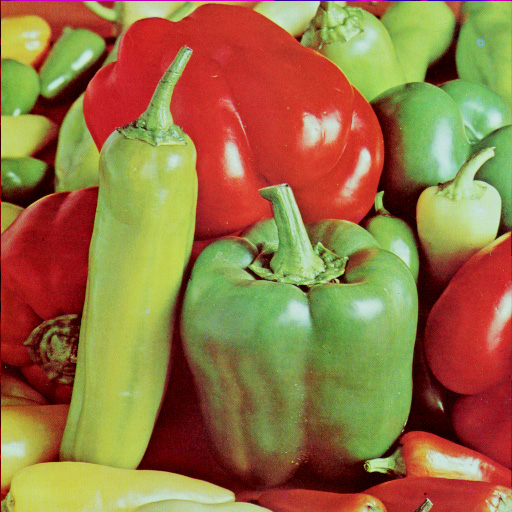
\includegraphics[width=5cm]{peppers.jpg}
\end{center}
\caption*{元画像}
\end{minipage}
\begin{minipage}{0.33\hsize}
\begin{center}
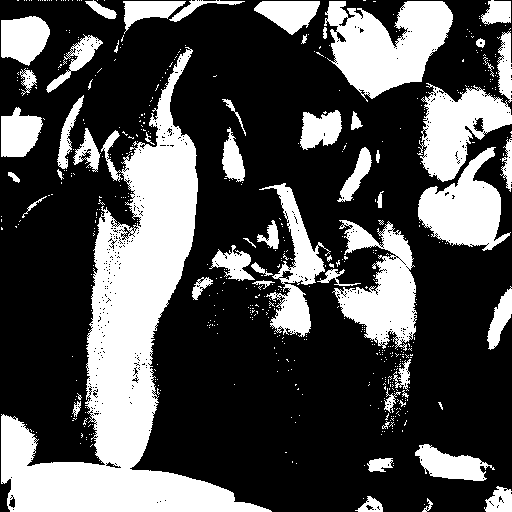
\includegraphics[width=5cm]{peppers_red_135.png}
\end{center}
\caption*{赤抽出 閾値:123}
\end{minipage}
\begin{minipage}{0.33\hsize}
\begin{center}
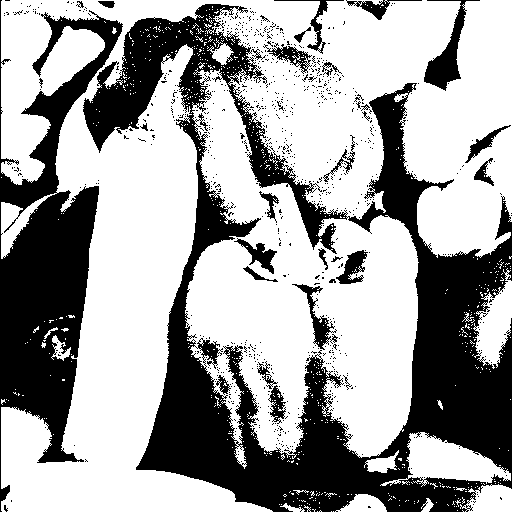
\includegraphics[width=5cm]{peppers_green_95.png}
\end{center}
\caption*{緑抽出 閾値:95}
\end{minipage}
\end{tabular}
\end{center}
\end{figure}
考察:\\
二値化の式は、
\begin{equation}
	g(i,j)=
\left\{\begin{array}{ll}
255 & (f(i,j) > thresh) \\
0 & (f(i,j) \leqq  thresh)
\end{array}
\right.
\end{equation}
である。実際の処理ではそれぞれのRGB値の平均を求めてそれを閾値と比べている。

閾値95で抽出できるピーマンの部分はRGB合計が285以上に集まっており、黒で抽出した赤色はRGB
合計が369以下に集まっていると考えられる。

このことから、ピーマンの抽出は閾値95で白、パプリカ
は閾値123で黒で抽出するのが最適である。

\subsection*{課題3-1:画像の縮小}
PPM ファイル “zoneplate256.ppm” の画像を入力として
「平均値」を用いて画像を縦横それぞれ 1/4 倍のサイズ(64 × 64)に縮小せ
よ.縮小した結果画像をレポートに貼り,画質について考察せよ.
また,その結果をダウンサンプリング法と比較せよ.ただし,縮小倍率は 1/4 倍
とする.

プログラム

ダウンサンプリング法:
\begin{lstlisting}
	/* 縮小1(ダウンサンプリング) */
void scale_down_DS(ColorImage *outimage, const ColorImage *inimage)
{
    int i,j;
	int wide,high;//wide : 横の拡大率 high : 縦の拡大率
	printf("縦の縮小率を入力\n>>>");
	scanf("%d",&high);
	printf("横の縮小率を入力\n>>>");
	scanf("%d",&wide);
	//演算
	for(i=0;i < outimage -> width; i++){//一行ずらす
		for(j=0;j < outimage -> height; j++){//一列ずらす
			outimage -> r[i][j] = inimage -> r[(int)(i*wide)][(int)(j*high)];//位置の入れ替え、赤
			outimage -> g[i][j] = inimage -> g[(int)(i*wide)][(int)(j*high)];//位置の入れ替え、緑
			outimage -> b[i][j] = inimage -> b[(int)(i*wide)][(int)(j*high)];//位置の入れ替え、青
		}
	}
}
\end{lstlisting}

平均値を用いた縮小:
\begin{lstlisting}
void scale_down_Mean(ColorImage *outimage, const ColorImage *inimage)
{
  int i,j,k,l;//i : 横の画素値 j:縦の画素値 k:横の平均を取る画素の座標 l:縦の平均を取る画素の座標
	int wide,high;//wide : 横の縮小率 high : 縦の縮小率
	int sumr,sumg,sumb;// sum: 画素地の合計
	float red=0,green = 0,blue=0; //画素値を一時的に格納
	//倍率入力
	printf("縦の縮小倍率を入力\n>>>");
	scanf("%d",&high);
	printf("横の縮小倍率を入力\n>>>");
	scanf("%d",&wide);
	//演算
	for(i=0;i < outimage -> width; i++){//一行ずらす
		for(j = 0;j < outimage -> height; j++){//一列ずらす
			sumr = 0;sumg = 0 ; sumb = 0;//sum値の初期化
			for(k = 0;k < wide;k++){
				for(l = 0;l < high; l++){
					if(!(i*wide+k >= inimage -> width || j*high+l >= inimage -> height)){
						sumr = sumr + (inimage -> r[i*wide+k][j*high+l]); //r値の合計を変数sumrに格納
						sumg = sumg + (inimage -> g[i*wide+k][j*high+l]); //g値の合計を変数sumgに格納
						sumb = sumb + (inimage -> b[i*wide+k][j*high+l]);//b値の合計を変数sumbに格納
					}
				}
			}
			red = sumr / (wide * high); //平均を取り、変数sumrに格納
			green = sumg / (wide * high); //平均を取り、変数sumgに格納
			blue = sumb / (wide * high); //平均を取り、変数sumbに格納
			//変更を反映。
			outimここge -> r[i][j] = red;
			outimage -> g[i][j] = green;
			outimage -> b[i][j] = blue;
		}
	}
}
\end{lstlisting}

実行結果:\\
ダウンサンプリング法で縮小した画像は中心の円の画像パターンが繰り返されているのに対し、
平均値を用いた縮小では比較的元画像に対して忠実なまま縮小された。
%横に3枚の画像(jpg/png)表示
\begin{figure}[H]
\begin{center}
\begin{tabular}{c}
\begin{minipage}{0.33\hsize}
\begin{center}
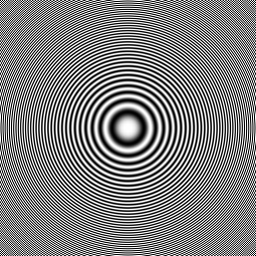
\includegraphics[width=5cm]{zoneplate256.jpg}
\end{center}
\caption{元画像}
\label{}
\end{minipage}
\begin{minipage}{0.33\hsize}
\begin{center}
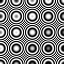
\includegraphics[width=5cm]{scale_down_DS.jpg}
\end{center}
\caption{ダウンサンプリング}
\label{}
\end{minipage}
\begin{minipage}{0.33\hsize}
\begin{center}
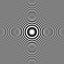
\includegraphics[width=5cm]{scale_down_4.jpg}
\end{center}
\caption{平均値を用いた縮小}
\label{}
\end{minipage}
\end{tabular}
\end{center}
\end{figure}
※組版の関係上、同じ大きさで表示しているが、実際は図2,3は図1の1/16の大きさである。

考察:\\
ダウンサンプリングの計算式は、縦横の縮小倍率をそれぞれ$M,N$、
縦横の大きさをそれぞれ$H,W$とすると、
\begin{equation}
	g(i,j)=f(Mi,Nj), 0 \leqq i < H , 0 \leqq j < W
\end{equation}
また、平均値を用いた縮小の計算式は、
\begin{equation}
	g_{L}(i,j)=\frac{1}{MN}\sum_{k=0}^{M-1}\sum_{l=0}^{N-1}f_{L}(Mi+k,Nj+l)
\end{equation}
平均値を用いた縮小では、縮小倍率に応じた範囲内にある画素を平均して出力画素としている。
画素数が減る分、画質は悪くなる。しかし一部だけでなく周辺の画素も加味した値であるため
出力する画素に偏りが生じにくく、ダウンサンプリング法と比較して元画像に忠実な縮小画像が出力できる。

一方ダウンサンプリング法では縮小倍率の倍数の位置にある画素のみ取り出し、出力画素
とする。このためダウンサンプリングの画像が表しているのは、「4の倍数の座標に位置する画素だけ集めた画像」
である。このため元画像のようにパターンを含む画像を縮小しようとすると、同じような
模様が並んでいる画像になる。

\subsection*{課題3-2:画像の拡大}
線形補間法を用いて画像を縦横それぞれ 2 倍のサイズ(512 × 512)
に拡大せよ.拡大した結果画像はレポートに貼り,画像について考察せよ.
また, その結果を最近傍法と比較せよ.

プログラム:

線形補完法:
\begin{lstlisting}
	/* 拡大3(線形補間) */
void scale_up_IP(ColorImage *outimage, const ColorImage *inimage)
{
	int i,j;
	int wide,high;//wide : 横の拡大率 high : 縦の拡大率
	float sep_top_r,sep_top_g,sep_top_b; //sep_top : 上の内分点の画素値
	float sep_bot_r,sep_bot_g,sep_bot_b; //sep_bot:下の内分点の画素値
	float alpha,beta; //alpha : i/wideの小数値 beta:j/highの小数値
	int i_childa,j_childa; //i_childa : i/wide  j_childa : j/high
	//倍率読み込み
	printf("縦の拡大率を入力\n>>>");
	scanf("%d",&high);
	printf("横の拡大率を入力\n>>>");
	scanf("%d",&wide);
	//演算
	for(i=0;i < outimage -> width - wide; i++){//一行ずらす
		for(j=0;j < outimage -> height -high; j++){//一列ずらす
			i_childa = i/wide;
			j_childa = j/high;
			//i/wide、j/wideが整数値であるとき
			if(i%wide == 0 && j%high == 0){
				outimage -> r[i][j] = inimage -> r[(int)i_childa][(int)j_childa];
				outimage -> g[i][j] = inimage -> g[(int)i_childa][(int)j_childa];
				outimage -> b[i][j] = inimage -> b[(int)i_childa][(int)j_childa];
			}
			//i/wide,j/wideが整数値でないとき
			else{
				//補完座標
				i_childa = floor(i_childa);
				beta = i/wide - i_childa;
				j_childa = floor(j_childa);
				alpha = j/high - j_childa;
				//上の内分点
				sep_top_r = (1-alpha)*inimage->r[(int)i_childa][(int)j_childa] + alpha* inimage -> r[(int)i_childa][(int)(j_childa+1)];
				sep_top_g = (1-alpha)*inimage->g[(int)i_childa][(int)j_childa] + alpha* inimage -> g[(int)i_childa][(int)(j_childa+1)];
				sep_top_b = (1-alpha)*inimage->b[(int)i_childa][(int)j_childa] + alpha* inimage -> b[(int)i_childa][(int)(j_childa+1)];
				//下の内分点
				sep_bot_r = (1-alpha)*inimage->r[(int)(i_childa+1)][(int)j_childa] + alpha* inimage -> r[(int)(i_childa+1)][(int)(j_childa+1)];
				sep_bot_r = (1-alpha)*inimage->r[(int)(i_childa+1)][(int)j_childa] + alpha* inimage -> r[(int)(i_childa+1)][(int)(j_childa+1)];
				sep_bot_r = (1-alpha)*inimage->r[(int)(i_childa+1)][(int)j_childa] + alpha* inimage -> r[(int)(i_childa+1)][(int)(j_childa+1)];
				//補完演算
				outimage -> r[i][j] = (1-beta)*sep_top_r + beta * sep_bot_r;
				outimage -> g[i][j] = (1-beta)*sep_top_g + beta * sep_bot_g;
				outimage -> b[i][j] = (1-beta)*sep_top_b + beta * sep_bot_b;
			}
		}
	}
}
\end{lstlisting}

最近傍法:
\begin{lstlisting}
	void scale_up_IP(ColorImage *outimage, const ColorImage *inimage)
{
	int i,j;
	int wide,high;//wide : 横の拡大率 high : 縦の拡大率
	float sep_top_r,sep_top_g,sep_top_b; //sep_top : 上の内分点の画素値
	float sep_bot_r,sep_bot_g,sep_bot_b; //sep_bot:下の内分点の画素値
	float alpha,beta; //alpha : i/wideの小数値 beta:j/highの小数値
	int i_childa,j_childa; //i_childa : i/wide  j_childa : j/high
	//倍率読み込み
	printf("縦の拡大率を入力\n>>>");
	scanf("%d",&high);
	printf("横の拡大率を入力\n>>>");
	scanf("%d",&wide);
	//演算
	for(i=0;i < outimage -> width - wide; i++){//一行ずらす
		for(j=0;j < outimage -> height -high; j++){//一列ずらす
			i_childa = i/wide;
			j_childa = j/high;
			//i/wide、j/wideが整数値であるとき
			if(i%wide == 0 && j%high == 0){
				outimage -> r[i][j] = inimage -> r[(int)i_childa][(int)j_childa];
				outimage -> g[i][j] = inimage -> g[(int)i_childa][(int)j_childa];
				outimage -> b[i][j] = inimage -> b[(int)i_childa][(int)j_childa];
			}
			//i/wide,j/wideが整数値でないとき
			else{
				//補完座標
				i_childa = floor(i_childa);
				beta = i/wide - i_childa;
				j_childa = floor(j_childa);
				alpha = j/high - j_childa;
				//上の内分点
				sep_top_r = (1-alpha)*inimage->r[(int)i_childa][(int)j_childa] + alpha* inimage -> r[(int)i_childa][(int)(j_childa+1)];
				sep_top_g = (1-alpha)*inimage->g[(int)i_childa][(int)j_childa] + alpha* inimage -> g[(int)i_childa][(int)(j_childa+1)];
				sep_top_b = (1-alpha)*inimage->b[(int)i_childa][(int)j_childa] + alpha* inimage -> b[(int)i_childa][(int)(j_childa+1)];
				//下の内分点
				sep_bot_r = (1-alpha)*inimage->r[(int)(i_childa+1)][(int)j_childa] + alpha* inimage -> r[(int)(i_childa+1)][(int)(j_childa+1)];
				sep_bot_r = (1-alpha)*inimage->r[(int)(i_childa+1)][(int)j_childa] + alpha* inimage -> r[(int)(i_childa+1)][(int)(j_childa+1)];
				sep_bot_r = (1-alpha)*inimage->r[(int)(i_childa+1)][(int)j_childa] + alpha* inimage -> r[(int)(i_childa+1)][(int)(j_childa+1)];
				//補完演算
				outimage -> r[i][j] = (1-beta)*sep_top_r + beta * sep_bot_r;
				outimage -> g[i][j] = (1-beta)*sep_top_g + beta * sep_bot_g;
				outimage -> b[i][j] = (1-beta)*sep_top_b + beta * sep_bot_b;
			}
		}
	}
}
\end{lstlisting}
\newpage
実行結果:\\		
元画像と線形補完法の画像を比較した結果、元画像の要素のほとんどを残したまま
拡大された画像が生成された。
%横に3枚の画像(jpg/png)表示
\begin{figure}[H]
\begin{center}
\begin{tabular}{c}
\begin{minipage}{0.33\hsize}
\begin{center}
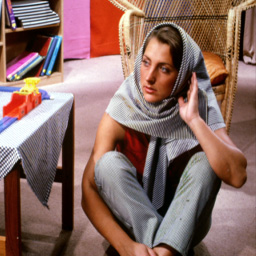
\includegraphics[width=5cm]{barbara256.jpg}
\end{center}
\caption{元画像}
\end{minipage}
\begin{minipage}{0.33\hsize}
\begin{center}
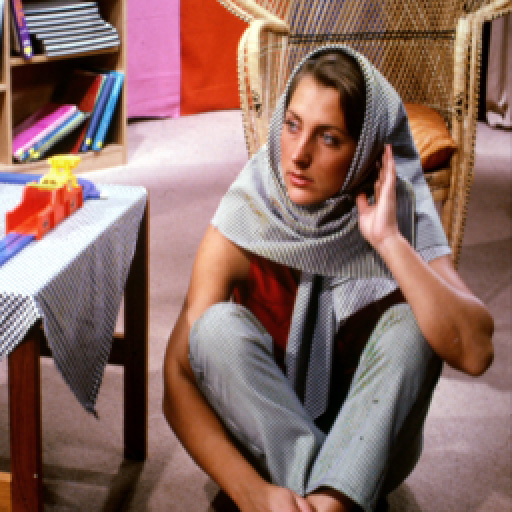
\includegraphics[width=5cm]{scale_up_NN_2.jpg}
\end{center}
\caption{線形補完法}
\end{minipage}
\begin{minipage}{0.33\hsize}
\begin{center}
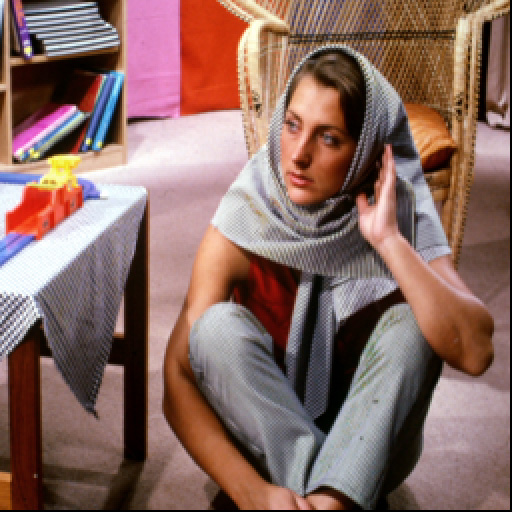
\includegraphics[width=5cm]{scale_up_IP_2.jpg}
\end{center}
\caption{最近傍法}
\end{minipage}
\end{tabular}
\end{center}
\end{figure}
※組版の関係上同じ大きさで載せているが、図5と図6は図4の4倍の大きさである。
\\
\\
考察:	
今回は2倍の拡大だったので、両者に大きな違いは見られなったが、
10倍など、倍率を大きくすると最近傍法は遠くの画素を取ることになり、粗い画像に
なると思われる。

一方で線形補完法は、線形に欠損画素を補完するという特性を持つため、
元画像に忠実な画像が作れる。

\subsection*{課題4:ガウシアンフィルタによる平滑化}
1. ガウシアンフィルタを実装し、σの値を 20 に固定しフィルタサイズを変え
たとき、出力画像はどのように変化するか? ただし、フィルタサイズは奇
数とする。
2. また、フィルタ長を 5 に固定しσの値を変えたとき、出力画像はどのように
変化するか?ただし、σは 0 より大きな整数とする。
上記について、結果から分かることを報告しその理由も述べよ。また、考察せ
よ。

プログラム:
\begin{lstlisting}
	void gaussian_filter(ColorImage *outimage, ColorImage *inimage, float sigma, int win_size) {
    /* 入力カラー画像inimageに対してガウシアンに基づく平滑化フィルタを計算し,出力用outimageに格納する.*/
    /* 必要であれば、変数宣言を適宜追加すること */
    /* ここにプログラムを挿入する */
    int i, j, k, l, L = (win_size - 1) / 2;
    float sumR = 0.0f, sumG = 0.0f, sumB = 0.0f;
    float InR,InG,InB; //それぞれ、入力画像の画素値。InR:赤 InG:緑 InB:青
    float w1 = 0.0f, sumW = 0.0f;
    for (i=0; i<outimage->height; i++) {
        for (j=0; j<outimage->width; j++) {
            sumR = 0.0f; sumG = 0.0f; sumB = 0.0f; sumW = 0.0f;//sumの初期化
            for (k=-L; k<=L; k++) {
                for (l=-L; l<=L; l++) {
                    /* 画像端では、画像の領域外にアクセスしないようにする */
                    if(i+k >= inimage -> width || j+l >= inimage -> height || i+k <= 0 || j+l <= 0){
                        //0埋め
                        InR = 0,InG = 0,InB = 0;
                    }
                    else{
                    //画素値の代替変数に画素値を代入。
                        InR = inimage -> r[i+k][j+l];
                        InG = inimage -> g[i+k][j+l];
                        InB = inimage -> b[i+k][j+l];
                    }
                    /* 重みを計算する */
                    w1 = exp(-((pow(k,2)+pow(l,2))/(2*pow(sigma,2))));
                    /* フィルタの係数の乗算 */
                    sumR += InR*w1;
                    sumG += InG*w1;
                    sumB += InB*w1;
                    sumW += w1;
                }
            }
        /* outimage[i][j]にフィルタの出力を格納する */
        outimage -> r[i][j] = sumR/sumW;
        outimage -> g[i][j] = sumG/sumW;
        outimage -> b[i][j] = sumB/sumW; 
        }

    }
}
\end{lstlisting}

問題1:

実行結果:\\
フィルタサイズを大きくするにつれて、画像にぼかしがかかった。
%横に4枚の画像(jpg/png)表示
\begin{figure}[H]
\begin{center}
\begin{tabular}{c}
\begin{minipage}{0.25\hsize}
\begin{center}
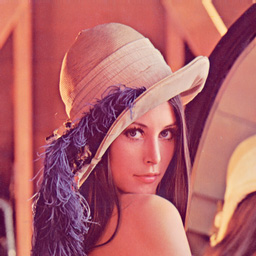
\includegraphics[width=4cm]{lena256.jpg}
\end{center}
\caption*{元画像}
\end{minipage}
\begin{minipage}{0.25\hsize}
\begin{center}
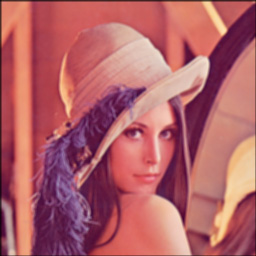
\includegraphics[width=4cm]{gauss_winsize_3.jpg}
\end{center}
\caption*{フィルタサイズ:2×2}
\end{minipage}
\begin{minipage}{0.25\hsize}
\begin{center}
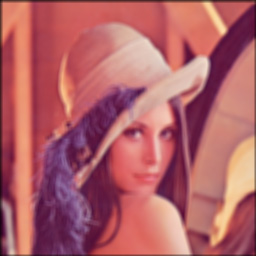
\includegraphics[width=4cm]{gauss_winsize_5.jpg}
\end{center}
\caption*{フィルタサイズ:4×4}
\end{minipage}
\begin{minipage}{0.25\hsize}
\begin{center}
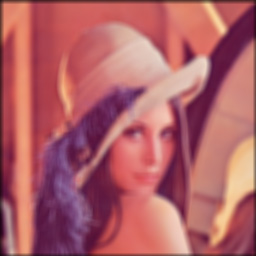
\includegraphics[width=4cm]{gauss_winsize_7.jpg}
\end{center}
\caption*{フィルタサイズ:6×6}
\end{minipage}
\end{tabular}
\end{center}
\end{figure}

考察:\\
このフィルタの数式は、
\begin{equation}
	g(i,j)=\frac{\sum_{k=-L}^{L}\sum_{l=-L}^{L}f(i+k,j+l)・\exp(-\frac{k^{2}+l^{2}}{2\sigma^{2}})}{\sum_{k=-L}^{L}\sum_{l=-L}^{L}\exp(-\frac{k^{2}+l^{2}}{2\sigma^{2}})}
	\label{gausian_filter}
\end{equation}
数式(\ref{gausian_filter})より、二次元ガウス分布$\exp(-\frac{k^{2}+l^{2}}{2\sigma^{2}})$で重みづけした周辺画素の
平均を出力画素としている。より広い範囲を平均する程画像の重みの差が小さくなり、
画像のエッジが鈍る。それゆえに画像が平滑化され、ぼかしがかかったような画像が出力された。

問題2:

実行結果:\\
標準偏差の値が大きくなればなるほど画像がぼかされている。
%横に3枚の画像(jpg/png)表示
\begin{figure}[H]
\begin{center}
\begin{tabular}{c}
\begin{minipage}{0.33\hsize}
\begin{center}
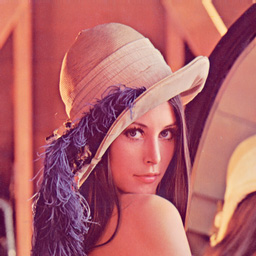
\includegraphics[width=5cm]{lena256.jpg}
\end{center}
\caption*{元画像}
\end{minipage}
\begin{minipage}{0.33\hsize}
\begin{center}
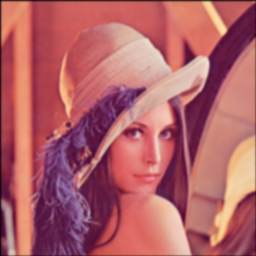
\includegraphics[width=5cm]{out_gauss_1.png}
\end{center}
\caption*{標準偏差:1}
\end{minipage}
\begin{minipage}{0.33\hsize}
\begin{center}
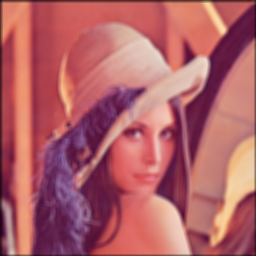
\includegraphics[width=5cm]{out_gauss_20.png}
\end{center}
\caption*{標準偏差:20}
\end{minipage}
\end{tabular}
\end{center}
\end{figure}

考察:\\
数式(\ref{gausian_filter})の二次元ガウス分布の部分$(\exp(-\frac{k^{2}+l^{2}}{2\sigma^{2}}))$
は画像のエッジの重みをあらわす。その分母である$2\sigma^{2}$が大きくなればなるほどエッジの重みが
全体的に軽くなり、エッジが鈍くなるから標準編差$\sigma$を増やしたとき、画像にぼかしがかかったようになった。

\subsection*{課題5:ラプラシアンフィルタによる鮮鋭化}
1. ラプラシアンフィルタによる鮮鋭化を実行するプログラム(コメント付き)
と処理結果画像を貼ること。
\\2. $K$の値を変えたときに鮮鋭化結果がどのように変化するか確認し、考察せよ。

プログラム:
\begin{lstlisting}
	void laplacian_sharpening(ColorImage *outimage, ColorImage *inimage, float K) {
    /* 入力カラー画像inimageに対してラプラシアンフィルタによる鮮鋭化結果を計算し,出力用outimageに格納する.*/
    /* ここにプログラムを挿入する */
    int i,j,k,l,L = 1; //参照範囲:winsize^2
    float sumR = 0.0f ,sumG = 0.0f ,sumB = 0.0f; //分母定義
    float InR,InG,InB; //inimageの画素地の代替変数
    int alap[3][3] = {{0,1,0},{1,-4,1},{0,1,0}}; //水平垂直方向のラプラシアンフィルタ
    for (i=0; i < outimage->height; i++) {
        for (j=0; j < outimage->width; j++) {
            sumR = 0.0f,sumG = 0.0f; sumB = 0.0f;
            for (k = -L; k <= L; k++)
            {
                for (l = -L; l <= L; l++)
                {
                    //segmentation fault対策
                    if(i+k >= inimage -> width || j+l >= inimage -> height || i+k <= 0 || j+l <= 0){
                        //0埋め
                        InR = 0,InG = 0,InB = 0;
                    }
                    else{
                        //画素値の代替変数に画素値を代入。
                        InR = inimage -> r[i+k][j+l];
                        InG = inimage -> g[i+k][j+l];
                        InB = inimage -> b[i+k][j+l];
                    }
                    //合計演算
                    sumR += alap[k+1][l+1] * InR;
                    sumG += alap[k+1][l+1] * InG;
                    sumB += alap[k+1][l+1] * InB;
                }
            }
            //画像演算 K:定数。
            outimage -> r[i][j] = inimage -> r[i][j] - K * sumR;
            outimage -> g[i][j] = inimage -> g[i][j] - K * sumG;
            outimage -> b[i][j] = inimage -> b[i][j] - K * sumB;
        }
    }
}
\end{lstlisting}

実行結果:\\
元の画像はエッジが鈍く、若干ぼやけた感じだが、エッジを足し合わせたことで船や周辺の
景色の輪郭がくっきりするようになっている。また、Kが大きくなるほど顕著である。
%横に3枚の画像(jpg/png)表示
\begin{figure}[H]
\begin{center}
\begin{tabular}{c}
\begin{minipage}{0.33\hsize}
\begin{center}
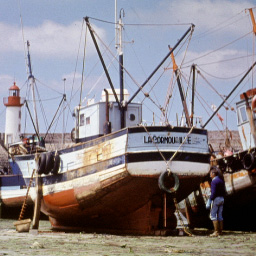
\includegraphics[width=5cm]{niceboat.jpg}
\end{center}
\caption{元画像}
\end{minipage}
\begin{minipage}{0.33\hsize}
\begin{center}
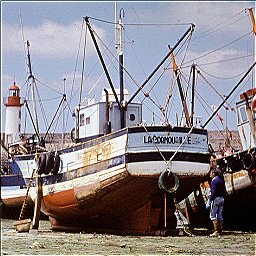
\includegraphics[width=5cm]{lap_k_p5.jpg}
\end{center}
\caption{K=0.5}
\end{minipage}
\begin{minipage}{0.33\hsize}
\begin{center}
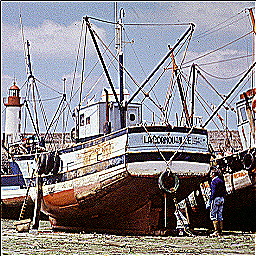
\includegraphics[width=5cm]{lap_k_2.jpg}
\end{center}
\caption{K=2}
\end{minipage}
\end{tabular}
\end{center}
\end{figure}

考察:\\
ラプラシアンフィルタによる鮮鋭化の計算式は、
\begin{gather}
	g(i,j)=f(i,j)-K\sum_{k=-L}^{L}\sum_{l=-L}^{L}a^{Lap}_{k,l}・f(i+k,j+l)\\
	a^{Lap}_{k,l}=\begin{bmatrix}
		0 & 1 & 0 \\
		1 & -4 & 1 \\
		0 & 1 & 0
	\end{bmatrix}
	\label{a^Lap}
\end{gather}
である。(\ref{a^Lap})はラプラシアンフィルタのカーネルである。(\ref{a^Lap})×周辺画素
の和は画素値と周辺画素の差、すなわちエッジである。そのエッジをK回足しこむので、よりエッジが
鋭くなり、Kの値を大きくするほどくっきりとした画像ができる。

\section{考察}
課題を総ざらいすると、最近傍法、線形補完には図形と方程式を利用するし、鮮鋭化には
線形代数学を利用する。ましてや画像データ自体が行列である。画像処理は数学の応用形
といった色合いが強いといったことがわかる。
\section{感想}
画像処理関係の授業と聞き、始めは機械学習を想像したのだが、骨のあるC言語でプログラミング
でき、自らのレベルも上げることができたように思う。また,segmentation faultなどのエラーに
できるだけ独力で立ち向かったが、これがさらに自分の画像処理に対する理解を深めたと考える。
また、レポート執筆中に考察を考えるのに苦労し、それに時間がかかった。この先どんなに難し
いプログラミング言語に出会ったとしても日本語より難しい言語は存在しないだろうと考える。
うんこ。
% !TEX root = main.tex
% !TEX root = main.tex

%%%%%%%%%% 参考文献 %%%%%%%%%%%%%%%%%%%%%%%%%%%%%%%%%%%%%%%%%%%%%%%%%%%
\begin{thebibliography}{99}
	\newcounter{num}
	\setcounter{num}{2}
	\bibitem{第三回講義スライド}第三回講義スライド
	\begin{verbatim}
		https://lms.kitakyu-u.ac.jp/pluginfile.php/275630/mod_resource/content/3/%E7%AC%AC3%E5%9B%9E%E8%AC%9B%E7%BE%A9%E3%82%B9%E3%83%A9%E3%82%A4%E3%83%89.pdf
	\end{verbatim}
	\bibitem{第四回講義スライド}第四回講義スライド
	\begin{verbatim}
		https://lms.kitakyu-u.ac.jp/pluginfile.php/276705/mod_resource/content/1/%E7%AC%AC4%E5%9B%9E%E8%AC%9B%E7%BE%A9%E3%82%B9%E3%83%A9%E3%82%A4%E3%83%89.pdf
	\end{verbatim}
	\bibitem{第七回講義スライド}第七回講義スライド
	\begin{verbatim}
		https://lms.kitakyu-u.ac.jp/pluginfile.php/280118/mod_resource/content/3/%E7%AC%AC7%E5%9B%9E%E8%AC%9B%E7%BE%A9%E3%82%B9%E3%83%A9%E3%82%A4%E3%83%89%EF%BC%88%E9%85%8D%E5%B8%83%E7%94%A8_p14%E3%80%8115%E8%A8%82%E6%AD%A3%E7%89%88%EF%BC%89.pdf
	\end{verbatim}
\end{thebibliography}
\end{document}